\documentclass[12pt]{article}
\usepackage{graphicx,psfrag,epsf}
\usepackage{enumerate}
\usepackage{natbib}
\usepackage{amsfonts}
\usepackage{amsmath}
\usepackage{float}
\usepackage{amsthm}
\usepackage{xcolor}
\usepackage{amssymb,mathabx}
\usepackage{algorithm, algpseudocode}
\usepackage[utf8]{inputenc}
\usepackage[english]{babel}
\newtheorem{theorem}{Theorem}
\newtheorem{lemma}[theorem]{Lemma}
\newtheorem{proposition}[theorem]{Proposition}
\newcommand{\blind}{0}
\addtolength{\oddsidemargin}{-.75in}%
\addtolength{\evensidemargin}{-.75in}%
\addtolength{\textwidth}{1.5in}%
\addtolength{\textheight}{1.3in}%
\addtolength{\topmargin}{-.8in}%

\input{mymacros.tex}

\begin{document}


%\bibliographystyle{plain}

\def\spacingset#1{\renewcommand{\baselinestretch}%
{#1}\small\normalsize} \spacingset{1}


%%%%%%%%%%%%%%%%%%%%%%%%%%%%%%%%%%%%%%%%%%%%%%%%%%%%%%%%%%%%%%%%%%%%%%%%%%%%%%

\if0\blind
{
  \title{\bf Efficient MCMC for Markov jump processes parameters}
  \author{  
   %  Vinayak Rao\thanks{
    %The authors gratefully acknowledge}\hspace{.2cm}\\
    %Department of Statistics, Purdue University\\
    %and \\
    Boqian Zhang \\
    Department of Statistics, Purdue University\\
    Vinayak Rao\\
    Department of Statistics, Purdue University\\
    }
  \maketitle
} \fi

\if1\blind
{
  \bigskip
  \bigskip
  \bigskip
  \begin{center}
    {\LARGE\bf Title}
\end{center}
  \medskip
} \fi

\bigskip
\begin{abstract}
Markov jump processes (MJPs) are continuous-time stochastic processes that 
find wide application in a variety of fields.  Inference for MJPs typically proceeds via Markov chain Monte Carlo, 
the state-of-the-art being a recent auxiliary variable Gibbs sampler proposed
in~\cite{RaoTeh13}. This algorithm was designed for the situation where
the MJP parameters are known, and Bayesian inference over unknown parameters
is typically carried out by incorporating this into a larger Gibbs 
sampler. %In many situations, the MJP trajectory and parameters can exhibit
%strong coupling, and 
This strategy of alternately sampling parameters given path, and 
then path given parameters can result in poor mixing. In this 
work, we propose a simple, elegant and novel algorithm to address this 
problem. Our scheme brings Metropolis-Hastings (MH) approaches 
for discrete-time hidden Markov models (HMMs) to the continuous-time
setting. Our proposed solution also ties up some of the loose ends 
in~\cite{RaoTeh13}, and provides a complete and clean recipe for 
parameter and path inference in MJPs. In our experiments, we 
demonstrate superior performance over Gibbs sampling, as well as 
other approaches like particle Markov chain Monte 
Carlo~\cite{Andrieu10}.
\end{abstract}
\noindent%
{\it Keywords:}  Markov jump process, MCMC, Metropolis-Hasting, Bayesian inference

\spacingset{1.45}

\section{Introduction}
\label{sec:intro}
Markov jump processes (MJPs) are continuous-time stochastic processes that
have found wide application in fields like computational chemistry~\cite{gillespie97}, 
population genetics~\cite{FearnSher2006}, mathematical finance~\cite{Elliott06}, 
queuing theory~\cite{Breuer2003}, artificial intelligence~\cite{XuShe10} and
social-network analysis~\cite{pan2016markov}. %The references above have
MJPs have been used to model the state of a chemical reaction, the state 
of a queuing network, segmentation of a strand of DNA, user activity on social 
media, among many others.

MJPs model temporal evolution in continuous-time, resulting in 
realistic, mechanistic, and interpretable models. %, often amenable to mathematical analysis. 
These same dynamics however raise computational
challenges in statistical applications, where given partial and noisy 
measurements, one has to make inferences over the latent MJP 
trajectory as well as any system parameters. Such
inference is complicated by two facts: one cannot {\em a priori} 
bound the number of state transitions, and the state-transition times themselves
are continuous-valued. This is in contrast to the situation with
{\em discrete-time} hidden Markov models. %and trajectory inference for 
%MJPs typically proceeds via Markov chain Monte Carlo. 
The state-of-the-art inference method for MJPs is an auxiliary variable Gibbs sampler proposed 
in~\cite{RaoTeh13}, we will henceforth refer to this as the {\algname} 
algorithm. The {\algname} algorithm was designed to sample paths when the MJP parameters
are known. Parameter inference is typically carried out by 
incorporating it into an outer Gibbs sampler that also simulates
parameters given the currently sampled trajectory. 

In many situations, the MJP trajectory and parameters can exhibit 
strong coupling, so that a Gibbs sampler that alternately samples path given
parameters, and then parameters given path can mix poorly.  
In this work, we propose a Metropolis-Hastings framework to address
this issue. Our proposed solution is simple and elegant, additionally,
it ties up some of the loose ends in the Rao-Teh algorithm.
In our experiments, we demonstrate superior 
performance over Gibbs sampling, as well as other approaches like 
particle Markov chain Monte Carlo~\cite{Andrieu10}.

\section{Markov jump processes (MJPs)} 
Formally, a Markov jump process~\cite{Cinlar1975} is a right-continuous 
piecewise-constant stochastic process $S(t)$ taking values in a countable, and 
usually finite state space $\cS$ (see Figure~\ref{fig:naive_mh}, top-left).
For simplicity, we will assume $N$-states, with $\cS = \{1,\ldots,N\}$. Then, 
an MJP is parameterized by two quantities, an $N$-component probability vector 
$\pi_0$ and a rate-matrix $A$. The former gives the distribution over states at 
the initial time (which without loss of generality we assume is $0$), while 
the latter is an $N \times N$-matrix governing the dynamics of the system.  An 
off-diagonal element $A_{ij}$, for some $i \neq j$ gives the rate at 
which the system transitions from state $i$ to $j$. We write $A_i$ for the 
negative of the $i$th diagonal element $A_{ii}$. For an MJP,
$A_i = -A_{ii} = \sum_{j \neq i} A_{ij}$, so that the rows of $A$ sum to $0$.  
$A_i$ gives the total rate at which the system leaves state $i$ for any other state.
To simulate an MJP trajectory over an interval $[0,\cT]$, one follows 
Gillespie's algorithm~\cite{gillespie97}: 
first sample an initial state $s_0$ from the distribution $\pi$, and
then defining $t_0 = t_{curr} = 0$ and $k = 0$, repeat the following two steps while
$t_{curr} < \cT$:
\begin{itemize}
  \item Sample a wait-time $\Delta t_k$ from an exponential distribution with rate 
    $A_{s_k}$.  Set $t_{k+1} = t_{curr} = t_{k} + \Delta t_k$.
    The MJP remains in state $s_k$ until time $t_{k+1}$.
  \item At the end of this time, jump to a new state $s_{k+1} \neq s_k$ with 
    probability equal to $A_{s_ks_{k+1}}/A_{s_k}$. Set $k=k+1$.
\end{itemize}
The times $T=(t_0, \cdots, t_{|T| })$ and states 
$S=(s_0, \cdots, s_{|T| })$ define the MJP path $S(t)$.

\subsection{Structured rate matrices}
In general, the rate matrix $A$ has $N(N-1)$ free parameters,
giving transition rates between every distinct pair of states. 
In typical applications, especially when large state-spaces
are involved, this $N \times N$ matrix is determined by a much smaller
set of parameters. We will write these as $\theta$, with
$A$ a deterministic function of these parameters: 
$A \equiv A(\theta)$. The parameters $\theta$ are often more 
interpretable than the elements of $A$ and correspond directly to
physical, biological or environmental parameters of interest. 
For example:
\begin{description}
  \item[The immigration-death process] This MJP is governed
    by two parameters: an arrival rate $\alpha$ and a death-rate
    $\beta$. The state space $\cS$ represents the size of a 
    population or the capacity of a queue. New individuals
    enter according to a rate-$\alpha$ Poisson process,
    so off-diagonal elements $A_{i,i+1}$ all equal $\alpha$.
    Each individual dies %(or each job completes) 
    at a rate $\beta$, so the system moves from state $i$ to 
    $i-1$ with rate $A_{i,i-1}=i\beta$.
    All other transitions have rate $0$, so that $\theta = (\alpha,\beta)$,
    and $A(\theta)$ is a tri-diagonal matrix.
  \item[Birth-death processes] This variant of the
    earlier MJP moves from state $i$ 
    to $i+1$ with rate $i\alpha$, with growth-rate proportional to 
    population size. Again, 
    $\theta=(\alpha,\beta)$.
  \item[Codon substitution models] Such models %are used in genetics
    characterize transition-rates between nucleotides or codons at a 
    DNA or RNA locus % on a DNA or RNA molecule 
    over evolutionary time. In the simplest case,
    all transitions have the same rate~\cite{jukescantor69}, 
    requiring just a single parameter. Other models categorize transitions 
    into groups, for instance `synonymous' transitions that continue to 
    encode the same amino acid, and `nonsynonymous' transitions giving 
    a new amino acid.  These have their own rates, and as 
    there are $61$ codons, this model results in a 
    $61\times 61$ transition matrix determined by 2 parameters. More refined 
    models~\cite{goldman1994codon} can introduce additional parameters. 
    %however the 
    %number of parameters is still significantly smaller than the general case.
\end{description}


\section{Bayesian inference for MJPs}
In realistic situations, one only observes the MJP trajectory at
a finite set of times, and typically, these observations themselves
are noisy. There are then two challenges than the practitioner
faces:
\begin{itemize}
  \item What is the MJP trajectory underlying the observations?
  \item What are the unknown parameters governing the MJP dynamics?
\end{itemize}

\subsection{Trajectory inference for MJPs}
This problem was addressed in~\cite{RaoTeh13}, and extended to a broader 
class of MJPs (as well as other jump processes like semi-Markov jump processes
) in~\cite{RaoTeh12}. Both these schemes are centered on an alternate
approaches to sampling MJP trajectories by introducing auxiliary
{\em thinned} candidate jump ideas. \cite{RaoTeh13} follows a classical
approach called uniformization, while in~\cite{RaoTeh12}, this was
extended to a more general dependent thinning approach. We outline
the latter below.

Recall that the diagonal elements of the rate matrix $A_i$ give the 
rate at which the MJP leaves state $i$ for any other state. Importantly,
the system is set up so that self-transitions cannot occur. Now,
for each parameter $A_i$, introduce an additional parameter $B_i \ge A_i$;
\cite{RaoTeh12} suggest setting $B_i = 2 A_i$. Assuming the system is
in state $i$, we sample a {\em candidate} transition time from an
exponential, not with rate $B_i$. At this time, the system remains in 
its current state with probability $1-A_i/B_i$. With the remaining 
probability, the system transitions to a new state, and as with
Gillespie's algorithm, we move to state $j \neq i$ with probability
proportional to $A_{ij}$. In~\cite{RaoTeh12}, it was shown that
trajectories sampled this way have the same distribution as trajectories
sampled according to Gillespie's algorithm.

Introducing the thinned variables allowed~\cite{RaoTeh13} to develop
a novel and efficient MCMC sampler. The algorithm proceeds as follows:\\
\textbf{Given the MJP trajectory $(S,T)$, sample a new set of thinned 
candidate times $U$}: \cite{RaoTeh12} show that these thinned events
are distributed as a piecewise-constant inhomogeneous Poisson process
with intensity $B_{S(t)}-A_{S(t)}$.\\
\textbf{Given the thinned and actual transition times $(T \cup U)$
    from the last iteration, sample a new trajectory}:
    Conditioned on the skeleton $T \cup U$, the set of candidate jump
    times is fixed, and trajectory inference reduces to inference for
    the familiar discrete-time hidden Markov model (HMM) with transition
    matrix $B$. Between any two consecutive time points, the system
    remain in a fixed state, with the likelihood for a state $i$ consisting
    of two parts: the likelihood of all observations falling in that 
    interval multiplied by a term $B_i\exp(-B_i\Delta t)$.

    ~\cite{RaoTeh12} show that the resulting Markov chain targets
    the desired posterior distribution over trajectories, and is 
    ergodic for any choice of $B$ with $B_i$ strictly greater than
    $A_i$.

\section{Parameter inference for MJPs}
In practice, the MJP parameters themselves are unknown: often,
these are the quantities of primary interest. A Bayesian approach
places a prior over these unknown variables, and follows a
Gibbs sampling approach to draw samples from the posterior:
for an arbitrary initialization, sample a trajectory from the
conditional $p(S(t)|X,\theta)$, and then, sample a new $\theta$
from the conditional $p(\theta|X,S(t))$. This distribution depends
on a set of sufficient statistics of the MJP trajectory: how
much time is spent in each state, and the number of transitions
between each pair of states. Given these, a new parameter set
can be sampled using any Markov kernel such as a Metropolis-Hastings
update, a Hamiltonian Monte Carlo update, or in special circumstances,
$\theta$ can be directly sampled from its conditional distribution.

Such conditional updates however come with a well known limitations:
when the paths and parameters are stongly coupled, the resulting
Gibbs sampler can be very inefficient, exploring parameter and
path space very sluggishly. In Figure~\ref{fig:conf1} we show
both the distribution of a component of $\theta$ conditioned
only on the observations, and conditioned on both the observations 
as well as a realization of the MJP trajectory: observe how much
more concentrated the latter is compared to the former. The
coupling is strengthened for longer and longer trajectories, so
that the Gibbs sampler can mix very poorly for situations with
long observation periods, even if the observations themselves are
sparse and uninformative.

For the discrete-time situation, this problem of parameter-trajectory can 
be circumvented by marginalizing out the MJP trajectory and directly 
carrying out inference over the parameters using a Metropolis-Hastings 
algorithm.  This scheme exploits the fact that the forward-backward 
algorithm used to sample a new trajectory retures the marginal probability 
of the observations $p(X|\theta)$ as a by product. This resulting 
algorithm them proceeds as follows:

\begin{itemize}
  \item Propose a new parameter $\theta^*$ from some proposal distribution
    $q(\theta*|\theta)$
  \item Run the forward pass of the forward-backward algorithm to 
    obtain the marginal likelihood of the observations, $p(X|\theta^*)$
  \item Accept this according to the usual Metropolis-Hastings acceptance
    probability.
  \item If desired, as new trajectory sample can be obtained by
    completing the backward pass of the forward-backward algorithm.
\end{itemize}

Naively calculating this marginal probability for the continuous-time
situation is not straightforward: this requires matrix-exponentials
to integrate out the now infinite number of paths, and this operation
is expensive, loses sparsity in the structure of the rate matrix,
and involves expensive computations that scale with the number of
observations rather than the actual dynamics of the system of interest.
In \cite{RaoTeh13}, the authors demonstrate the benefits of the
uniformization approach over such matrix exponential-based approaches,
and it is important to develop similar approaches for parameter inference.

The the key idea of the dependent-thinning approach of~\cite{RaoTeh13} is
to alternate a discrete-time HMM sampling step with a step that
samples a new random grid. This naturally suggests incorporating
the MH update step outlined earlier in a similar algorithm that also
updates parameters. As we will show, this approach does not quite
work, despite marginalizing out the MJP state the dependence of the
random grid on the MJP parameters can still slow down mixing.

\section{\Naive\ parameter inference via Metropolis-Hastings}
The idea of the Rao-Teh algorithm~\cite{RaoTeh13} is to simplify
computations by conditioning on the
random grid $W$.
%by combining extant transition times $T$ with a set of 
%thinned candidate transition times $U$, sampled from a rate-$(\Omega-A_{S(t)})$ 
%Poisson process. 
This suggests conditioning on $W$ to update
the parameters as well, following discrete-time scheme from
algorithm~\ref{alg:disc_time_mh}.
%The resulting scheme updates $\theta$ conditioned on the random 
%grid, but with the trajectory integrated out 
In particular, given $W$, discard all state information, and propose a 
new parameter $\vartheta$ from $q(\vartheta|\theta)$. 
%now conditioning on the set of times $W$.
To calculate the MH-acceptance probability $\min\left(1,
\frac{p(X|W,\vartheta)p(W|\vartheta)p(\vartheta)q(\theta|\vartheta)}
     {p(X|W,\theta)p(W|\theta)p(\theta)q(\vartheta|\theta)}\right)$, 
make a forward pass over $W$, and calculate 
$p(X|W,\theta)$ and $p(X|W,\vartheta)$. % as in algorithm~\ref{alg:disc_time_mh}.
After accepting or rejecting $\vartheta$, the new $\theta$ can be used in
a backward pass that samples a new trajectory. Then discard all 
self-transitions and repeat; algorithm~\ref{alg:MH_naive}, and 
figure~\ref{fig:naive_mh} in the appendix sketch this out.
\vspace{-.1in}
\begin{algorithm}[H]
   \caption{\Naive\  MH for parameter inference for MJPs }
   \label{alg:MH_naive}
  \begin{tabular}{l l}
   \textbf{Input:  } & \text{Observations $X$}, 
                       \text{the previous MJP path $S(t) = (S, T)$ and parameters $\theta$}.\\ 
                     & \text{A  Metropolis-Hasting proposal $q(\cdot | \theta)$}.\\
   \textbf{Output:  }& \text{A new MJP trajectory $S'(t) = (S', T')$, 
                            new MJP parameters $\theta'$}.\\
   \hline
   \end{tabular}
   \begin{algorithmic}[1]
     \State Set $\Omega \boqian{\equiv} \Omega(\theta) > \max_s{A_s(\theta)}$ for
     some function $\Omega(\cdot)$ (e.g.\ $\Omega(\theta) = 
      2\max_s A_s(\theta))$.
      \State Sample virtual jumps $U\subset[t_{start}, t_{end}]$ from a 
      Poisson process with piecewise-constant rate 
      $R(t) = (\Omega - A_{S(t)})$. 
    Set $W = T \cup U$ and discard MJP state information.
      \State Propose $\vartheta \sim q(\cdot| \theta)$.
          The acceptance probability is given by 
          \begin{align*}
          \alpha &=  1 \wedge \frac{p(W,\vartheta| y)}{p(W, \theta| y)} \frac{q(\theta|\vartheta)}{q(\vartheta|\theta)}
          =  1 \wedge \frac{p(y| W,\vartheta) p(W | \vartheta)p(\vartheta)}{p(y|W, \theta)p(W | \theta)p(\theta)} \frac{q(\theta|\vartheta)}{q(\vartheta|\theta)}.
          \end{align*}
    \State For both $\theta$ and $\vartheta$, make a forward pass through the 
    elements of $W$, sequentially updating the distribution over states at 
    $w \in W$ given observations upto $w$. 
    For any $\theta$, the Markov transition matrix 
    $B(\theta)$ equals $I + \frac{A(\theta)}{\Omega(\theta)}$ while the initial distribution
      over states is $\pi_0$. The likelihood of state $s$ at step $i$ is 
      $ L_i(s) = p(Y_{[w_i, w_{i + 1})} | S(t) = s , t \in [w_i, w_{i + 1})) = 
      \prod_{o: t_o \in [w_i, w_{i + 1})}p(y_{t_o} | s)$.
    At the end, we have 
    $p(X|W,\theta)$ and $p(X|W,\vartheta)$. Use these, and the fact that 
    $p(W|\theta)$ is Poisson-distributed to accept or reject the
    proposed $\vartheta$. Write the new state space
    as \boqian{$(W,\theta,\vartheta)$}.
    \State For the new parameter $\theta'$, make a backward pass through 
    the elements of
    $W$, sequentially assigning a state to each element of $W$. This
    completes the FFBS algorithm.
    \State Let $T'$ be the set of times in $W$ when the Markov chain changes state. Define $S'$ as the corresponding set of state values. Return $(S', T', \theta')$.
\end{algorithmic}
\end{algorithm}
\vspace{-.1in}
The resulting algorithm updates $\theta$ with the MJP trajectory integrated out, 
and will mix more rapidly than simple Gibbs. 
Note however that $\theta$ is updated {\em conditioned on
$W$}, and that
%determines not just the MJP trajectory $S(t)$.
%, and with $S(t)$ 
%marginalized out, the observations $X$. 
the distribution of $W$ depends on $\theta$: 
%These are the $p(W|\theta)$ terms
%in the acceptance probability; under uniformization, 
$W$ is a homogeneous
Poisson process with rate $\Omega(\theta) = 2 \max A(\theta)$. 
%who probability can
%calculated easily during the forward pass.
The fact that the MH-acceptance probability involves a $p(X|\theta)$ term
is inevitable, however in our experiments, we found that the $p(W|\theta)$
terms significantly effect acceptance. 
Any proposal that halves $\max A_s$ (and thus $\Omega$) will halve the
mean and variance of the distribution of the number of events in $W$, 
resulting in an extremely low acceptance probability.
The next section describes a way around this.



\section{An improved Metropolis-Hasting algorithm}
%\vspace{-.05in}
Our main idea is to symmetrize the probability of $W$ under the old and proposed parameters, so that $P(W|\theta)$ disappears from the acceptance ratio. 
Now, the probability of accepting a proposal $\vartheta$ depends only on the prior probabilities of $\theta$ and $\vartheta$, as well as how well they both explain the data.
This is in contrast to the previous algorithm, where one must also factor in how well each explains the current value of the grid $W$.
This results in a MCMC sampler that mixes significantly more fast. 
Since we also need do account for the probabilities $P(W|\theta)$, we also have a simpler MCMC scheme.
%This forms the main contribution of this paper.

\begin{algorithm} %[H]
   \caption{Symmetrized MH for parameter inference for MJPs }
   \label{alg:MH_improved}
  \begin{tabular}{l l}
   \textbf{Input:  } & \text{The observations $X$,}
                      \text{the MJP path $S(t) = (S, T)$, parameters $\theta$} and $\pi_0$.\\ 
                     & \text{A  Metropolis-Hasting proposal $q(\cdot | \theta)$}.\\
   \textbf{Output:  }& \text{A new MJP trajectory $S'(t) = (S', T')$, 
                            new MJP parameters $\theta'$}.\\
   \hline
   \end{tabular}
   \begin{algorithmic}[1]
     \State \textbf{Sample $\vartheta \sim q(\cdot| \theta)$}, and 
      set %$\Omega = \max_i A_i(\theta) + \max_i A_i(\theta^*)$. 
	$\Omega \assign \Omega(\theta) + \Omega(\vartheta)$ for some function 
    $\Omega(\theta) \ge \max_s A_s(\theta)$.
      %In the case of uniformization, we
      %have a single $\Omega$ for all states, with $\Omega = \max_i A_i(\theta) + \max_i A_i(\theta^*)$.
      %, with $h(\theta) > max_s{|A_s(\theta)|}$, $h(\theta^*) > max_s{|A_s(\theta^*)|}$ using some deterministic function $h$.
      \State \textbf{ Simulate the thinned times $U$ } from a rate-$(\Omega-A_{S(t)})$ Poisson process : 
\begin{align*}
  U \sim \text{PoissProc}(\Omega - A_{S(t)}) 
\end{align*}
    \State Set $W = T \cup U$ and discard MJP states $S$. The MCMC state is now 
    $(\theta,\vartheta, W)$.
 %   \State \textbf{MH proposal}: The current MCMC state-space is $(W,\theta,\vartheta)$. 
 %   Propose swapping $\theta$ and $\vartheta$, so the new state-space is $(W,\vartheta,\theta)$. 
 %    Accept with probability 
 %    $ \text{acc} 
 %      =  1 \wedge \frac{P(X| W,\vartheta,\theta)P(\vartheta)q(\theta|\vartheta)}
 %      {P(X| W,\theta, \vartheta)P(\theta) q(\vartheta|\theta)}.
 %      $
        \State \textbf{Forward pass:} Set $B(\theta,\vartheta) = I + \frac{A(\theta)}{\Omega(\theta, \vartheta)}$ and $\fwd^{\theta, \vartheta}_0(\cdot) = \pi_0$.
    %Sequentially update $\fwd^{\theta,\vartheta}_i(\cdot)$ at $w_i \in W$ as: 
    $$\textbf{for } i=1\rightarrow |W|\textbf{ do:} \quad \fwd^{\theta,\vartheta}_i(s') = \sum_{s \in \cS} \ell_{i-1}(s) \cdot \fwd^{\theta,\vartheta}_{i-1}(s)\cdot B_{ss'}(\theta,\vartheta), \quad \forall s' \in \cS.\qquad\qquad\quad $$
    Similarly, for $B(\vartheta,\theta) = I + \frac{A(\vartheta)}{\Omega(\vartheta, \theta)}$, calculate $\fwd^{\vartheta,\theta}_i(\cdot)$ for all $w_i \in W$.
    \State \textbf{Accept/reject}: The current MCMC state is $(W,\theta,\vartheta)$. 
    Propose to swap $\theta$ and $\vartheta$, %so the new state-space is $(W,\vartheta,\theta)$. 
     and accept with probability 
     $
   %  \texttt{acc} =  
     1 \wedge \frac{P(X| W,\vartheta,\theta)P(\vartheta)q(\theta|\vartheta)}
        {P(X| W,\theta, \vartheta)P(\theta) q(\vartheta|\theta)}.
        $
        Here, $P(X|W,\theta,\vartheta) = \sum_{s \in \cS} \fwd^{\theta,\vartheta}_{|W|}(s)$, and $P(X|W,\vartheta,\theta) = \sum_{s \in \cS} \fwd^{\vartheta,\theta}_{|W|}(s)$.
    Write the new MCMC state as $(W,\theta',\vartheta')$.
    \State \textbf{Backward pass:}
    Set $v_{|W|} \sim \bck^{\theta',\vartheta'}_{|W|}(\cdot)$, where $\bck^{\theta',\vartheta'}_{|W|}\!(s) \propto \fwd^{\theta',\vartheta'}_{|W|}\!(s)\cdot\ell_{|W|}(s) \quad \forall s \in \cS.$ 
    %For the new transition matrix $B(\theta',\vartheta')$,     
    $$\hspace{-.15in} \textbf{for } i=(|W|-1)\rightarrow 0\textbf{ do:} \ v_i \sim \bck^{\theta',\vartheta'}_i\!(\cdot), \text{where } 
    \bck^{\theta',\vartheta'}_i\!(s) \propto \fwd^{\theta',\vartheta'}_i\!(s)\cdot B_{sv_{i+1}}(\theta',\vartheta') \cdot \ell_i(s)  \ \forall s \in \cS.$$
    
%    Sample a path $\tilde{V}$, from a discret-time Markov chain with $|W| + 1$ steps, using FFBS algorithm. The transition matrix of the Markov chain is $B = (I + \frac{A(\tilde{\theta})}{\Omega})$ while the initial distribution over states is $\pi_0$. The likelihood of state $s$ at step $i$ is 
%    $$ L_i(s) = P(Y_{[w_i, w_{i + 1})} | S(t) = s \; for\; t \in [w_i, w_{i + 1})) = \prod_{j: t_j \in [w_i, w_{i + 1})}p(y_{t_j} | S(t_j) = s).$$\\
%%(i.e. $V(i) \sim P(V |  \theta(i), W(i - 1), y).$) Then delete all the virtual jumps to get $S(i), T(i) .$\\
    \State Let $T'$ be the set of times in $W$ when $V$ changes state. Define $S'$ as the corresponding set of state values. Return $(S', T', \theta')$.
\end{algorithmic}
\end{algorithm}


\setlength{\unitlength}{0.8cm}
  \begin{figure}[h!]
  \centering
  \begin{minipage}[!hp]{0.45\linewidth}
  \centering
    \includegraphics [width=0.90\textwidth, angle=0]{figs/plot0.pdf}
      \end{minipage}
  \begin{minipage}[hp]{0.45\linewidth}
  \centering
    \includegraphics [width=0.90\textwidth, angle=0]{figs/plot1.pdf}
    \vspace{-0 in}
  \end{minipage}
  \begin{minipage}[hp]{0.45\linewidth}
  \centering
    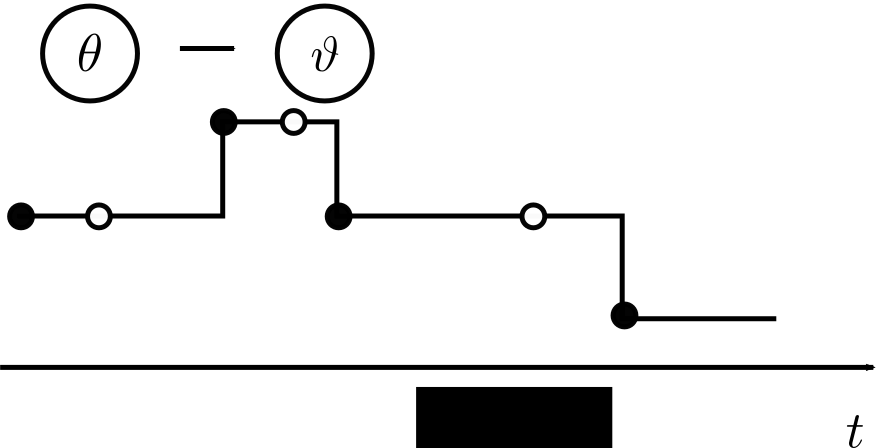
\includegraphics [width=0.90\textwidth, angle=0]{figs/plot2.pdf}
    \vspace{-0 in}
  \end{minipage}
  \begin{minipage}[hp]{0.45\linewidth}
  \centering
    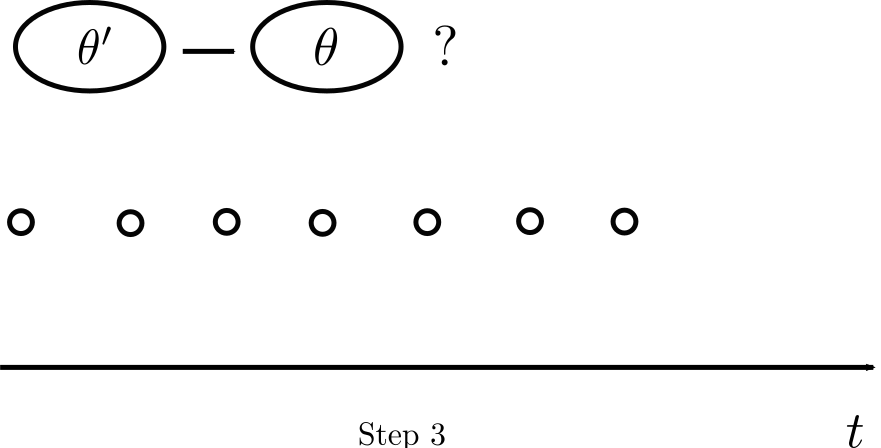
\includegraphics [width=0.90\textwidth, angle=0]{figs/plot3.pdf}
    \vspace{-0 in}
  \end{minipage}
% \begin{minipage}[hp]{0.45\linewidth}
% \centering
%   \includegraphics [width=0.70\textwidth, angle=0]{figs/plot4.pdf}
%   \vspace{-0 in}
% \end{minipage}
  \begin{minipage}[hp]{0.45\linewidth}
  \centering
    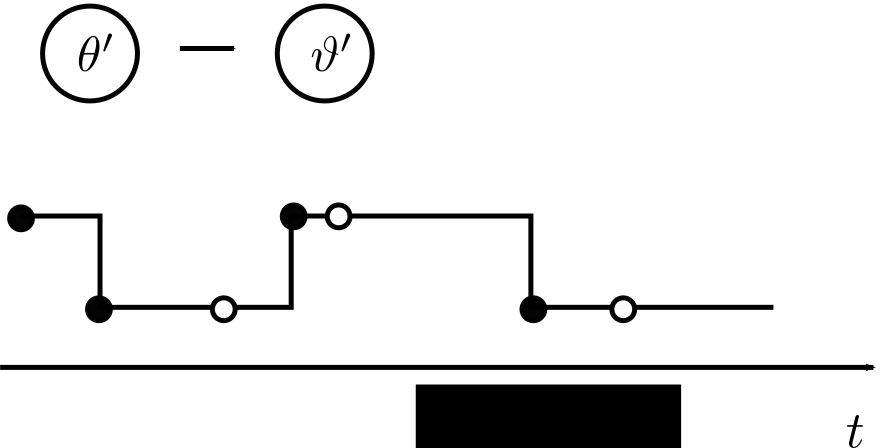
\includegraphics [width=0.90\textwidth, angle=0]{figs/plot5.pdf}
    \vspace{-0 in}
  \end{minipage}
  \begin{minipage}[hp]{0.45\linewidth}
  \centering
    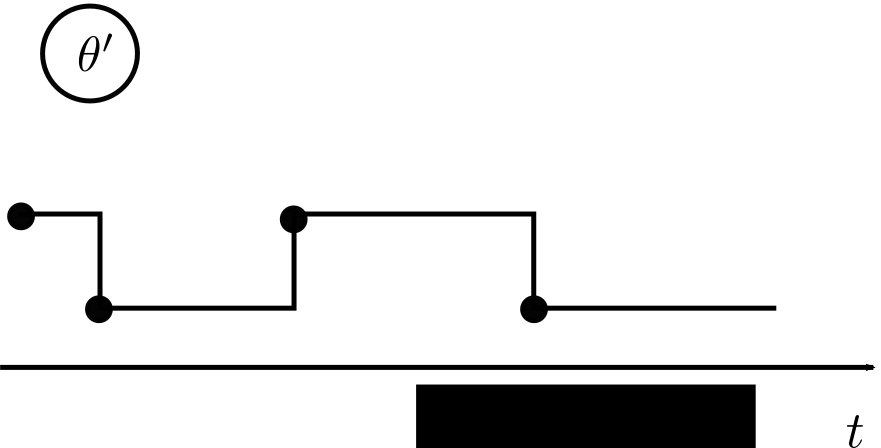
\includegraphics [width=0.90\textwidth, angle=0]{figs/plot6.pdf}
  \end{minipage}
    \caption{Proposed MH algorithm: Steps 0-3: Starting with a trajectory and parameter $\theta$, simulate an auxiliary parameter $\vartheta$, and then the thinned events
      $U$ from a rate $\Omega(\theta) + \Omega(\theta^*) - A_{S(t)}$ Poisson
      process. Step 4: Propose swapping $\theta$ and $\vartheta$. Step 5:
      Run a forward pass to accept or reject this proposal, and use the accepted
    parameter to simulate a new trajectory. Step 6: Discard $\vartheta'$ and the thinned events.} 
   \label{fig:MH_improved}
  \end{figure}
As before, the MCMC iteration begins with the pair $(S(t), \theta)$. 
Instead of simulating the Poisson events $U$, we first generate a new 
parameter $\vartheta$ from $q(\vartheta|\theta)$. Treat this as an 
auxiliary variable, so that the augmented space now is the triplet 
$(S(t), \theta,\vartheta)$. We pretend $S(t) \equiv (S,T)$ was sampled by  
uniformization, where the dominating Poisson rate $\Omega$ equals 
$(\Omega(\theta) + \Omega(\vartheta))$ instead of just $\Omega(\theta)$:
recall any choice greater than $\max_s A_s$ is valid.
Now the set of thinned events $U$ is piecewise-constant
Poisson with intensity $\Omega(\theta) + \Omega(\vartheta) - 
A_{S(t)}$. Following algorithm~\ref{alg:Unif_gibbs} or~\cite{RaoTeh13}, 
the {\em a priori} probability of the reconstructed set $W = U \cup T$, 
$P(W|\theta,\vartheta)$, is a homogeneous Poisson 
%the union of $U$ with the actual trajectory transition times $T$, 
process with rate $\Omega(\theta) + \Omega(\vartheta)$. Discard all 
MJP state information, so that the MCMC state space is $(W, \theta, \vartheta)$,
and propose swapping $\theta$ with $\vartheta$. 
Observe from
symmetry that the Poisson skeleton $W$ has the same probability both
before and after this proposal, so that unlike the previous scheme,
the ratio $P(W|\vartheta)/P(W|\theta)$ equals $1$.  This simplifies 
computation, and significantly improves mixing.
The acceptance probability 
%depends only on the probability of the observations
%under both set of parameters, %as we can use the forward-backward algorithm
%to calculate this. Our acceptance probability 
equals
$ 
  \min\left(1, \frac{P(X,\vartheta)q(\theta|\vartheta)}
   {P(X,\theta)q(\vartheta|\theta)}\right) = 
  \min\left(1, \frac{P(X|\vartheta)p(\vartheta)q(\theta|\vartheta)}
   {P(X|\theta)p(\theta)q(\vartheta|\theta)}\right).
   $
   The terms $P(X|\vartheta)$ and  $P(X|\theta)$ can be calculated by 
   running a forward pass of the forward-backward algorithm, and after
   accepting or rejecting the proposal, a new trajectory is sampled by
   completing the backward pass. Finally, the thinned events are
   discarded. Algorithm~\ref{alg:MH_improved} and 
   figure~\ref{fig:MH_improved} outline the details. 


%\subsection{Correctness of the proposed algorithm }
%\label{sec:verify2}
\begin{proposition}
  The sampler described in Algorithm~\ref{alg:MH_improved} has the posterior
  distribution $p(\theta,S(t)|X)$ as its stationary distribution.
\end{proposition}
\begin{proof}
  Suppose that at the start of the algorithm, we have a pair $(\theta,S(t))$ from
  the posterior distribution $p(\theta,S(t)|X)$. Introducing $\theta^*$
  from $q(\theta^*|\theta)$ results in a triplet whose marginal over the first
  two variables is still $p(\theta,S(t)|X)$.

  Sampling $U$ from a Poisson process with rate $\Omega(\theta) +
  \Omega(\theta^*) - A_{S(t)}(\theta)$, results in a random grid $W = T \cup U$
  that is distributed according to a rate $\Omega(\theta) + \Omega(\theta^*)$
  Poisson process (Proposition 2 in~\cite{RaoTeh13}). Discarding all state 
  information results in a triplet $(W,\theta,\theta^*)$ with probability
  proportional to $p(\theta)q(\theta^*|\theta)p(W|\theta,\theta^*)
  p(X|W,\theta,\theta^*)$.

Next we propose swapping $\theta$ and $\theta^*$, since this
is a deterministic proposal, the MH-acceptance probability is given by
$$\alpha = 1 \wedge \frac{p(\theta^*)q(\theta|\theta^*)p(W|\theta^*,\theta)
p(X|W,\theta^*,\theta)}{p(\theta)q(\theta^*|\theta)p(W|\theta,\theta^*)
p(X|W,\theta,\theta^*)}$$
The term $p(W|\theta,\theta^*)$ is just a Poisson process with rate $\Omega(\theta)+
\Omega(\theta^*)$, so that $p(W|\theta,\theta^*) = p(W|\theta,\theta^*)$. The
two terms $p(X|W,\theta,\theta^*)$ and $p(X|W,\theta^*,\theta)$ are obtained
at the end of a forward pass over $W$ using discrete-time transition matrices
$B(\theta,\theta^*) = \left(I + \frac{A(\theta)}{\Omega(\theta)+\Omega(\theta^*)}\right)$ 
and $B(\theta^*,\theta) = \left(I + \frac{A(\theta^*)}{\Omega(\theta)+\Omega(\theta^*)}\right)$. 

Calling the parameters 
after the accept step $(\tilde{\theta}, \tilde{\theta}^*)$, we have that
$(\tilde{\theta}, \tilde{\theta}^*,W)$ has the same distribution as
$(\theta, \theta^*,W)$.
Finally, following Lemma 1 in~\cite{RaoTeh13}, using the matrix 
$B(\tilde{\theta},\tilde{\theta}^*)$ to make a backward pass through $W$,
and discarding the self-transitions results in a trajectory $(\tilde{S}(t)$
distributed according to $A(\tilde{\theta})$. Discarding the auxiliary parameter
$\tilde{\theta}^*$ results is a pair $(\tilde{\theta},\tilde{S}(t))$ from
the posterior.
% \begin{align*}
%  p(y, W, S, T, \theta, \theta^*) &= p(\theta) q(\theta^* | \theta) P(S,T| \theta, \theta^*) P(W| S, T, \theta, \theta^*)P(y | S, T, \theta, \theta^*)\\
%  &=p(\theta) q(\theta^* | \theta) P(S,T| \theta) P(W| S, T, \theta, \theta^*)P(y | S, T).
% \end{align*}
% The marginal distribution of $(y, S, T, \theta, \theta^*)$ and $(y, S, T, \theta)$ as follows.\\
% \begin{align*}
%  p(y, S, T, \theta, \theta^*) &= p(\theta) q(\theta^* | \theta) P(S,T| \theta, \theta^*)P(y | S, T, \theta, \theta^*)\\
%  &=P(y, S, T, \theta) q(\theta^* | \theta).
% \end{align*}
% \begin{align*}
%  p(y, S, T, \theta) &= p(\theta)P(S,T| \theta)P(y | S, T, \theta).
% \end{align*}
% So the conditional distribution over $\theta^*$ given $(y, S, T, \theta)$ is $q(\theta^* | \theta)$. And the conditional distribution over W given $(y, S, T, \theta, \theta^*)$  is $P(W | S, T, \theta, \theta^*)$, which is actually the distribution of Non Homogeneous Poisson Process with piecewise constant rate $h(\theta) + h(\theta^*) - A_{S(t)}(\theta)$.\\
% Thus the Step 1 + Step 2 is actually equivalent to sampling from the conditional distribution $P(\theta^* , W| S, T, \theta, y)$.\\
% The Step 3 + Step 4 satisfy the detailed balance condition. The reason is as follows.
% \begin{align*}
% &P((W, S, T, (\theta, \theta^*)) \rightarrow (W, S^*, T^*, (\theta^*, \theta))) P(S,T, (\theta, \theta^*) | W, y)\\
% &= (1 \wedge \frac{P((\theta^*,\theta) | W, y)}{P((\theta,\theta^*) | W, y)})P(S^*, T^* | W, (\theta^*, \theta), y)P(S, T | W, (\theta, \theta^*), y)P((\theta, \theta^*) | W, y)\\
% &= P((W, S^*, T^*, (\theta^*, \theta)) \rightarrow (W, S, T, (\theta, \theta^*))) P(S^*,T^*, (\theta^*, \theta) | W, y)
% \end{align*} 
% Therefore the stationary distribution of this MCMC sampler is $P(W, S, T, (\theta, \theta^*) | y)$. Thus the stationary distribution of $(S, T, \theta)$ is the corresponding marginal distribution $P(S, T, \theta | y)$.  
\end{proof}




\section{Generic Exponential Model}~
\begin{algorithm}[!ht]
   \caption{Generic Gibbs sampling for MJPs for Gamma priors}
   \label{alg:Generic Gibbs}
\begin{algorithmic}
   \State {\bfseries Input:} observations $y_{[t_0, t_{k+1})}$
   \State Initialize, $i = 0$
   \\ (a) Set $\alpha(0), \beta(0)$ arbitrarily and set current trajectory $[S,T](0)$ arbitrarily.\\
    (b) Uniformize $[S,T](0)$, to get virtual jumps $U$.
   \Repeat
   \For{$i=1$ {\bfseries to} $N$}
    \State (a) Sample $U(i) \sim P( U | \beta(i - 1), \alpha(i - 1), S(i - 1), T(i - 1), y)$.\\	
    \State (b) Use FFBS algorithm to  sample states given all the jump times(both true jumps and virtual jumps).
(i.e. $V(i) \sim P(V |  \beta(i - 1), \alpha(i - 1), W(i ), y).$) Then delete all the virtual jumps to get $S(i), T(i) .$\\
    \State (c) Propose $\beta^* \sim q(.| \beta(i -1))$.\\
      Set $\beta(i) = \beta^*$, with probability $P_{acc} = 1 \wedge \frac{P(\beta^* |S(i), T(i))}{P(\beta(i - 1) |S(i), T(i))} \frac{q(\beta(i - 1)|\beta^*)}{q(\beta^*|\beta(i - 1))}$;\\Otherwise set $\beta(i) = \beta(i-1)$.\\	  
    \State (d) Sample $\alpha(i) \sim P(. | \beta(i), S(i), T(i), y)$.\\ It is a $Gamma(\mu + N, \lambda + \sum_{0}^NF_{S_i}(\beta)(t_{i + 1} - t_i))$ distribution actually.\\
    \EndFor
    \Until{$ i = N$ }
 \end{algorithmic}
 \end{algorithm}
  \begin{figure}[H]
  \centering
  \begin{minipage}[!hp]{0.45\linewidth}
  \centering
    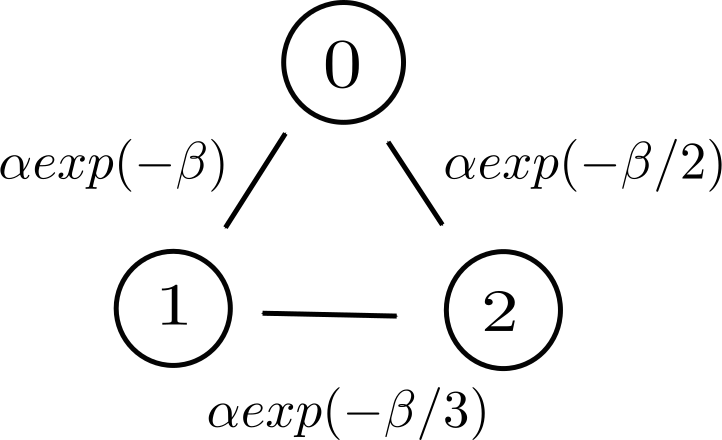
\includegraphics [width=0.70\textwidth, angle=0]{figs/exp_model.pdf}
      \end{minipage}
    \caption{exp model}
  \end{figure}

\noindent Assume: $S = [S_0,S_1, ...,S_N] \;, T = [t_0(t_{start}), t_1,...,t_N, t_{N+1}(t_{end})]$, and y as observations.\\
We consider a specific structure of rate matrix $A$. $A_{ij} = \alpha f_{ij}(\beta), \; i \neq j$. $A_{ii} = -\sum_{j \neq i} A_{ij}$. $0 \leq f_{ij} \leq 1$. Denote $F_i(\beta) = \sum_{j \neq i} f_{ij}(\beta)$.\\
\begin{align*}
P(s_0, S, T | \alpha, \beta) &= \pi_0(s_0)\prod_{i = 1}^N A_{S_{i - 1}S_i} \exp(- \int_{t_{start}}^{t_{end}} |A_{S(t)}| dt)\\
&= \pi_0(s_0) \alpha^N \prod_{i = 1}^N f_{S_{i - 1}S_i} \exp(-\alpha  \sum_{i = 0}^{N} F_{S_i}(\beta)(t_{i + 1} - t_i))\\
\end{align*}
We can assume the prior distributions of $\alpha, \beta$ are $p_1(\alpha)$ and $p_2(\beta)$.\\
Then the posterior distribution of parameters $\alpha, \beta$ will be as follows.\\
\begin{align*}
P(\alpha, \beta | s_0, S, T ) \propto \alpha^N \prod_{i = 1}^N f_{S_{i - 1}S_i} \exp(-\alpha  \sum_{i = 0}^{N} F_{S_i}(\beta)(t_{i + 1} - t_i)) p_1(\alpha)p_2(\beta)\\
\end{align*}
If we assume the priors of $\alpha$, $\beta$ are $Gamma(\mu, \lambda)$, $Gamma(\omega, \theta)$, then the posterior will have a simper form as follows. 
\begin{align*}
P(\alpha, \beta | s_0, S, T ) = C \alpha^{\mu + N - 1}\exp(-\alpha (\lambda + \sum_{i = 0}^{N} F_{S_i}(\beta)(t_{i + 1} - t_i))) \prod_{i = 1}^N f_{S_{i - 1}S_i}  \beta ^{\omega - 1} \exp(-\theta \beta)\\
\end{align*}
We notice that given $\beta,\; S,\; T$, $\alpha$ is distributed as a $Gamma$ distribution.\\
$\alpha | \beta, S, T, y  = \alpha | \beta, S, T \sim Gamma(\mu + N, \lambda + \sum_{0}^NF_{S_i}(\beta)(t_{i + 1} - t_i))$.\\
There is no conjugate distribution to sample $\beta \sim P(\beta| s_0, S, T)$. We will have to use Metropolis Hasting within Gibbs to sample $\beta$. The target distribution is the following one.
$$ P(\beta | S, T) = C \frac{\prod_{i = 1}^N f_{S_{i -1}S_i}(\beta)\beta^{\omega - 1} \exp(-\theta \beta)}{(\lambda + \sum_{i = 0}^{N} F_{S_i}(\beta)(t_{i + 1} - t_i))^{\mu + N}}.$$
Such doubling might slow the mixing of the Markov chain. We can apply our Metropolis Hasting algorithm on this model.
\subsection{Experiments}
In the following, we evaluate a Python implementation of our algorithms compared to other exact samplers which include Gibbs sampler and Particle MCMC sampler. We consider one special case when $f_{ij}(\beta) = \exp(-\beta / (i + j))$. We consider three different dimensions which are 3, 5, and 10 and three different k which are 1.5, 2, and 3. We generated random parameters $\alpha$, $\beta$ from prior distributions ($Gamma(3,2), Gamma(5, 2)$), and used these parameters to construct the transition matrix A. Then we generate an MJP trajectory with a uniform initial distribution over states and the transition matrix A. The state of this MJP trajectory was observed via a Normal distribution with mean equal to the value of state and variance 1, and the proposal kernel is a lognormal distribution with location parameter $\log(\theta_{old})$ and scale parameter$\sigma$. Posterior samples given the observations were produced by a Python implementation of our algorithm. 100 MCMC runs were performed, each run consisting of 10000 iterations except for Particle MCMC algorithm. For Particle MCMC, each run consists 3000 iterations while the number of particles can be 5, 10 or 20. We also explored the gradient information of the target distribution to apply Hamiltonian Monte Carlo with different step sizes and different numbers of leapfrog jumps. For HMC,  each run consists 20000 iterations while the numbers of leapfrog jumps can be 1, 3, 5, or 10, and the leapfrog stepsize can be  0.02, 0.05 and 0.1. For each run, the acceptance rates as well as the time spent was calculated, and effective sample sizes (ESSs) of MCMC sampling parameters) were calculated using R-CODA (Plummer et al., 2006). The overall ESS per unit time of a run is defined to be the mean ESS per unit time across all these ESSs per unit time.\\
Figure 1, 2 and 3 plot the overall  ESS per unit time against the variance of the proposal kernel per run, for different methods and different scaling parameters k($k = 1.5, 2, 3$) and different dimensions($p = 3, 5, 10$), where the  $\Omega = k \max(\Omega_{old}, \Omega_{new})$ when $k < 2$, or $\Omega = k (\Omega_{old} + \Omega_{new})$ when $k \leq 2$. We see that the improved MH algorithm is more efficient in these cases with respect to the overall ESS per unit time. We also see that increase the scaling parameter will decrease the efficiency of the improved MH algorithm respect to overall ESS per unit time, when $k > 2$. If we set $\Omega = 1.5 \max(\Omega_{old}, \Omega_{new})$, the performance of the improved MH will not be as good as the case we set $\Omega = 2(\Omega_{old} + \Omega_{new})$ when the proposal log variance is large.\\
Figure 4 shows the initial burn-in of a sampler with this setting for different initializations. The vertical axis shows the number of state transitions in the MJP trajectory of each iteration. This quantity quickly reaches its equilibrium value within a few iterations.\\

Figure 5 plots ESS per unit time a
Figure 6 plots ESS per unit time as observation interval and the number of observations both increase when the dimension is $3$ and the scaling parameter k is $2$. Gibbs sampler decreases faster than Metropolis Hasting Method, due to the doubling of MJP paths and the parameters. \\

Figure 7 plots ESS per unit time as observation interval increases with number of observations fixed, when the dimension is $3$ and the scaling parameter k is $2$.Gibbs sampler decreases faster than Metropolis Hasting Method, due to the doubling of MJP paths and the parameters. In addition Gibbs sampler decreases even more faster than previous case when the number of observations is not fixed. \\

Figure 8 plots ESS plots the overall  acceptance rate against the log variance of the proposal kernel per run for dimension $3$. 


  \begin{figure}%[b]
  \centering
  \begin{minipage}[!hp]{0.45\linewidth}
  \centering
    \includegraphics [width=0.70\textwidth, angle=0]{figs/exp_3_alpha.pdf}
      \end{minipage}
  \begin{minipage}[hp]{0.45\linewidth}
  \centering
    \includegraphics [width=0.70\textwidth, angle=0]{figs/exp_3_beta.pdf}
    \vspace{-0 in}
%    \caption{ESS/sec for exp model (beta, dim 3)}
     \label{fig:ESS_EXP_D3}
  \end{minipage}
    \caption{ESS/sec for exp model (dim 3). The left is for $\alpha$, and the right is for $\beta$.}
  \end{figure}
  \begin{figure}[H]
  \centering
  \begin{minipage}[hp]{0.45\linewidth}
  \centering
    \includegraphics [width=0.70\textwidth, angle=0]{figs/h_alpha.pdf}
      \end{minipage}
  \begin{minipage}[hp]{0.45\linewidth}
  \centering
    \includegraphics [width=0.70\textwidth, angle=0]{figs/h_beta.pdf}
      \end{minipage}

    \caption{HMC for dim 3}
  \end{figure}


  \begin{figure}%[b]
  \centering
  \begin{minipage}[hp]{0.45\linewidth}
  \centering
    \includegraphics [width=0.70\textwidth, angle=0]{figs/exp_5_alpha.pdf}
%    \caption{ESS/sec for exp model (alpha, dim 5)}
      \end{minipage}
  \begin{minipage}[hp]{0.45\linewidth}
  \centering
    \includegraphics [width=0.70\textwidth, angle=0]{figs/exp_5_beta.pdf}
    \vspace{-0 in}
%    \caption{ESS/sec for exp model (beta, dim 5)}
     \label{fig:ESS_EXP_D5}
  \end{minipage}
    \caption{ESS/sec for exp model (dim 5)}
  \end{figure}

  \begin{figure}%[b]
  \centering
  \begin{minipage}[hp]{0.45\linewidth}
  \centering
    \includegraphics [width=0.70\textwidth, angle=0]{figs/exp_10_alpha.pdf}
      \end{minipage}
  \begin{minipage}[!hp]{0.45\linewidth}
  \centering
    \includegraphics [width=0.70\textwidth, angle=0]{figs/exp_10_beta.pdf}
    \vspace{-0 in}
     \label{fig:ESS_EXP_D10}
  \end{minipage}
    \caption{ESS/sec for exp model (dim 10)}
  \end{figure}
  
  
  
  \begin{figure}%[b]
  \centering
  \begin{minipage}[hp]{0.45\linewidth}
  \centering
    \includegraphics [width=0.70\textwidth, angle=0]{figs/exp3_k2_path_transition.pdf}
    \caption{Trace plot of the number of MJP transitions for different initializatoins for exponential model.}
      \end{minipage}
  \end{figure}

  \begin{figure}%[b]
  \centering
  \begin{minipage}[hp]{0.45\linewidth}
  \centering
    \includegraphics [width=0.70\textwidth, angle=0]{figs/ESS_vs_t_alpha.pdf}
      \end{minipage}
  \begin{minipage}[hp]{0.45\linewidth}
  \centering
    \includegraphics [width=0.70\textwidth, angle=0]{figs/ESS_vs_t_beta.pdf}
    \vspace{-0 in}
     \label{fig:TSS}
  \end{minipage}
    \caption{Time Interval vs. ESS / sec}
  \end{figure}

  \begin{figure}%[b]  
  \centering
  \begin{minipage}[hp]{0.45\linewidth}
  \centering
    \includegraphics [width=0.70\textwidth, angle=0]{figs/ESS_vs_t_alpha_fixobservation.pdf}
    \end{minipage}
  \begin{minipage}[hp]{0.45\linewidth}
  \centering
    \includegraphics [width=0.70\textwidth, angle=0]{figs/ESS_vs_t_beta_fixobservation.pdf}
    \vspace{-0 in}
     \label{fig:TSS2}
  \end{minipage}
    \caption{Time Interval vs. ESS / sec (Number of observations is fixed)}
  \end{figure}
  \begin{figure}%[b]
  \centering
  \begin{minipage}[hp]{0.45\linewidth}
  \centering
    \includegraphics [width=0.70\textwidth, angle=0]{figs/acc_rate_exp_d3.pdf}
    \caption{Acceptance rate for exp model (dim 3)}
      \end{minipage}
  \end{figure}


\section{Immigration models with capacity}~
An $M/M/N/N$ queue is a stochastic process whose state space is the set $\{0, 1, 2, 3, ..., N - 1\}$ where the value corresponds to the number of customers in the system, including any currently in service. Arrivals occur at rate $\alpha$ according to a Poisson process and move the process from state $i$ to $i+1$. Service times have an exponential distribution with parameter $\beta$ in the $M/M/N/N$ queue. There are $N$ servers, which serve from the front of the queue. If there are less than $N$ jobs, some of the servers will be idle. Only $N$ customers can queue at any one time. Any further arrivals to the queue are considered "lost". 
  \begin{figure}[H]
  \centering
  \begin{minipage}[!hp]{0.6\linewidth}%0.45
  \centering
    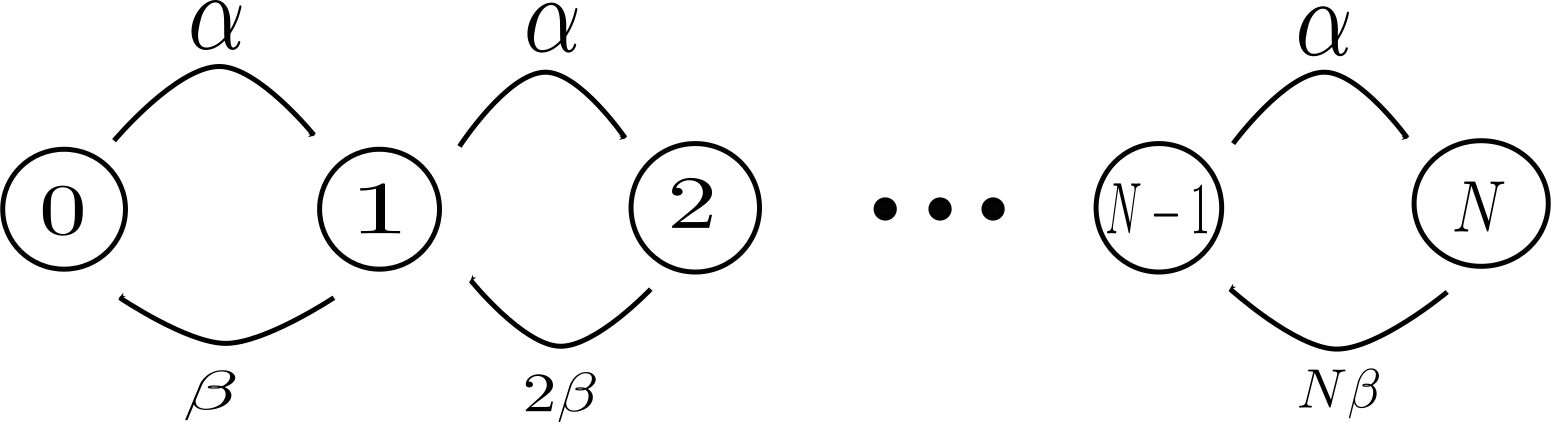
\includegraphics [width=1\textwidth, angle=0]{figs/queue_model.pdf}%0.70
      \end{minipage}
    \caption{exp model}
  \end{figure}

\noindent Assume: $S = [S_0,S_1, ...,S_N] \;, T = [t_0(t_{start}), t_1,...,t_N, t_{N+1}(t_{end})]$, and y as observations.\\
Now, let's consider a immigration model as follows. State space is $\{0, 1, 2, ..., N - 1\}$, representing the total population. The transition matrix is defined as follows. 
$$A_i =: A_{i,i} = -(\alpha + i\beta), \; \; i =0,1,...,N$$ $$A_{i, i+1} = \alpha, \; \; i =0,1,...,N-1,$$ $$A_{i, i-1}  = \beta, \; \;  i =1,...,N.$$
We already know the conditional density(given $\alpha,\; \beta$) of a MJP trajectory $(s_0, S, T)$ in time interval $[t_{start}, t_{end}]$, with $S=(s_1, s_2,..., s_k)$, $T=(t_1, t_2,..., t_k)$. 
$$f(s_0,S,T| \alpha, \beta) = \prod_{i=0}^{k-1} A_{s_i, s_{i+1}} \exp(\sum_{i=0}^{k} A_{s_i}(t_{i+1} - t_{i})), $$
where $t_0 = t_{start}$, $t_{k+1} = t_{end}.$\\
Let's denote some notations here.\\
$$U(s_0, S, T):= \sum_{i=0}^{k-1} \mathbb{I}_{\{s_{i+1} - s_i = 1\}}.$$
$$D(s_0, S, T):= \sum_{i=0}^{k-1} \mathbb{I}_{\{s_{i+1} - s_i = -1\}}.$$
Call them U and D for short.
Let's denote the total time when the trajectory state stays at state i as $\tau_i$, i.e. $\tau_i = \sum_{j=0}^{k} (t_{j+1} -t_j)\mathbb{I}_{\{s_j = i\}}$, then $\sum_{i=0}^k (t_{i+1} - t_i)s_i = \sum_{i=0}^N \tau_ii.$\\

$$f(s_0,S,T| \alpha, \beta) = \exp(-\alpha(t_{end} - t_{start}- \tau_N) )\alpha^U \cdot  \exp((-(\sum_{i=0}^k (t_{i+1} - t_i)s_i)\beta) \prod_{i=1}^N i^{\sum_{j=0}^{k-1}\mathbb{I}_{s_{j+1} = i -1 \;,  s_j = i} }   \beta^D$$\\
If we assume the prior of $\alpha$, and $\beta$ are $Gamma(\mu,\lambda)$, $Gamma(\omega, \theta)$, which are independent with each other. \\
$$p(\alpha) = \frac{\lambda^\mu}{\Gamma(\mu)}\alpha^{\mu -1}e^{-\lambda \alpha}. $$
$$p(\beta) = \frac{\theta^\omega}{\Gamma(\omega)}\beta^{\omega -1}e^{-\theta \beta}. $$
Then we can get the posterior distribution $$f(\alpha, \beta | s_0,S,T)$$ as follows.
$$ f(\alpha, \beta | s_0,S,T) \propto \exp(-(\lambda + t_{end} - t_{start}- \tau_N)\alpha) \alpha^{\mu + U -1} \cdot \exp(-(\sum_{i=0}^k (t_{i+1} - t_i)s_i + \theta)\beta) \beta^{\omega+ D -1}.$$
It means that the posterior distributions of $\alpha$, $\beta$ are still independent. \\
$\alpha | s_0,S,T$ is following $Gamma(\mu+ U,\lambda + t_{end} - t_{start}- \tau_N)$\\
$\beta | s_0,S,T$ is following $Gamma(\omega+ D,\theta + \sum_{i=0}^k (t_{i+1} - t_i)s_i)$, which is equivalent to $Gamma(\omega+ D,\theta +\sum_{i=0}^N \tau_ii)$\\
Such immigration models have perfectly conjugate posterior distributions when we assign $\gamma$ priors to $\alpha$ and $\beta$. We apply our Metropolis Hasting algorithms on such models to compare the performance with the performance of Gibbs Sampling algorithm.
\subsection{Experiments}
In the following, we evaluate a Python implementation of our algorithms compared to other exact samplers which include Gibbs sampler and Particle MCMC sampler. We consider three different dimensions which are 3, 5, and 10 and three different k which are 1.5, 2, and 3. We generated random parameters $\alpha$, $\beta$ from prior distributions ($Gamma(3,2), Gamma(5, 2)$), and used this to construct the transition matrix A. Then we generate an MJP trajectory with a uniform initial distribution over states. The state of this MJP trajectory was observed via a Normal distribution with mean equal to the value of state and variance 1, and posterior samples given the observations were produced by a Python implementation of our algorithm. 100 MCMC runs were performed, each run consisting of 10000(Varies among different dimensions) iterations. For each run, the number of transitions as well as the time spent was calculated, and effective sample sizes (ESSs) of these statistics (the number of independent samples with the same `information' as the correlated MCMC samples) were calculated using R-CODA (Plummer et al., 2006). The overall ESS of a run is defined to be the mean ESS across all these ESSs.

  \begin{figure}%[b]
  \centering
  \begin{minipage}[!hp]{0.45\linewidth}
  \centering
    \includegraphics [width=0.70\textwidth, angle=0]{figs/q_3_alpha.pdf}
      \end{minipage}
  \begin{minipage}[!hp]{0.45\linewidth}
  \centering
    \includegraphics [width=0.70\textwidth, angle=0]{figs/q_3_beta.pdf}
    \vspace{-0 in}
     \label{fig:ESS_Q_3}
  \end{minipage}
    \caption{ESS/sec for Immigration model (dim 3)}
  \end{figure}
  \begin{figure}%[b]
  \centering
  \begin{minipage}[!hp]{0.45\linewidth}
  \centering
    \includegraphics [width=0.70\textwidth, angle=0]{figs/q_5_alpha.pdf}
      \end{minipage}
  \begin{minipage}[!hp]{0.45\linewidth}
  \centering
    \includegraphics [width=0.70\textwidth, angle=0]{figs/q_5_beta.pdf}
    \vspace{-0 in}
     \label{fig:ESS_Q_5}
  \end{minipage}
    \caption{ESS/sec for Immigration model (dim 5)}
  \end{figure}

  \begin{figure}%[b]
  \centering
  \begin{minipage}[!hp]{0.45\linewidth}
  \centering
    \includegraphics [width=0.70\textwidth, angle=0]{figs/q_10_alpha.pdf}
      \end{minipage}
  \begin{minipage}[!hp]{0.45\linewidth}
  \centering
    \includegraphics [width=0.70\textwidth, angle=0]{figs/q_10_beta.pdf}
    \vspace{-0 in}
     \label{fig:ESS_Q_10}
  \end{minipage}
    \caption{ESS/sec for Immigration model (dim 10)}
  \end{figure}

\begin{figure}
  \begin{minipage}[!hp]{0.45\linewidth}
  \centering
    \includegraphics [width=0.70\textwidth, angle=0]{figs/q3_k2_path_transition.pdf}
    \vspace{-0 in}
    \caption{Trace plot of the number of MJP transitions for different initializatoins for immigration model.}
     \label{fig:ESS_EXP_TRANSITION}
  \end{minipage}
\end{figure}

  \begin{figure}%[b]
  \begin{minipage}[!hp]{0.45\linewidth}
  \centering
    \includegraphics [width=0.70\textwidth, angle=0]{figs/dist_alpha.pdf}
    \vspace{-0 in}
     \label{fig:dist_alpha}
  \end{minipage}
  \begin{minipage}[!hp]{0.45\linewidth}
  \centering
    \includegraphics [width=0.70\textwidth, angle=0]{figs/dist_beta.pdf}
    \vspace{-0 in}
     \label{fig:dist_beta}
  \end{minipage}
    \caption{density}
  \end{figure}

  \begin{figure}%[b]
  \begin{minipage}[!hp]{0.45\linewidth}
  \centering
    \includegraphics [width=0.70\textwidth, angle=0]{figs/hist_alpha.pdf}
    \vspace{-0 in}
     \label{fig:dist_alpha1}
  \end{minipage}
  \begin{minipage}[!hp]{0.45\linewidth}
  \centering
    \includegraphics [width=0.70\textwidth, angle=0]{figs/hist_beta.pdf}
    \vspace{-0 in}
     \label{fig:hist_beta}
  \end{minipage}
    \caption{test}
  \end{figure}
  

\section{DNA evolution JC69 model }~
  \begin{figure}[H]
  \centering
  \begin{minipage}[!hp]{0.45\linewidth}
  \centering
    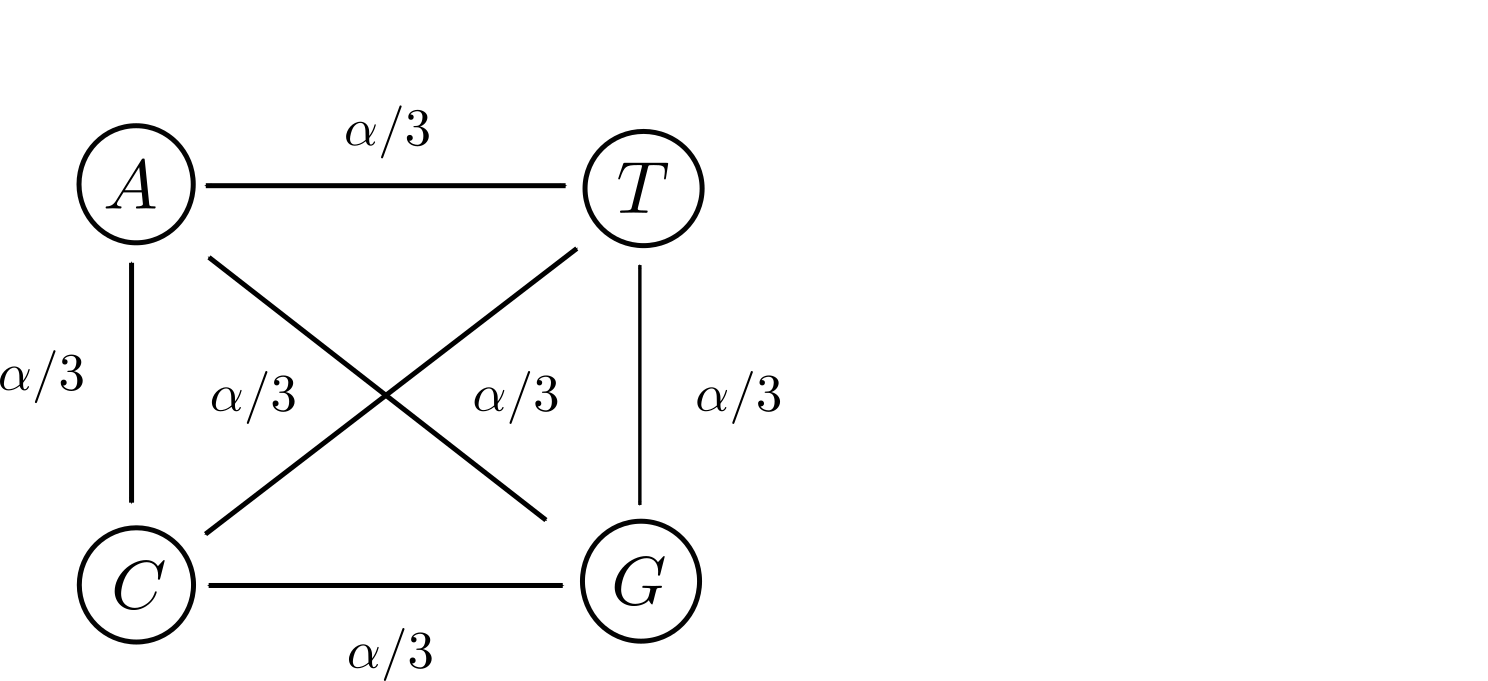
\includegraphics [width=0.70\textwidth, angle=0]{figs/jc_model.pdf}
      \end{minipage}
    \caption{exp model}
  \end{figure}

JC69 is the simplest substitution model. There are several assumptions. It assumes equal base frequencies and equal mutation rates. The only parameter of this model is $\alpha$. The overall substitution rate is therefore $3\alpha$. The state space is $\{1, 2, 3, 4\}$, representing $\{A, T, C, G\}$.\noindent Assume: $S = [S_0,S_1, ...,S_N] \;, T = [t_0(t_{start}), t_1,...,t_N, t_{N+1}(t_{end})]$, and y as observations.\\
$$A_i =: A_{i,i} = -3\alpha, \; \; i =0,1,...,N$$ $$A_{i, j} = \alpha, \; \; i \neq j.$$
If we assume the prior of $\alpha$ is $Gamma(\mu,\lambda)$\\
$$p(\alpha) = \frac{\lambda^\mu}{\Gamma(\mu)}\alpha^{\mu -1}e^{-\lambda \alpha} $$.
Then we can get the posterior distribution $$f(\alpha | s_0,S,T)$$ as follows.
$$ f(\alpha| s_0,S,T) \propto \exp(-(\lambda + 3(t_{end} - t_{start}))\alpha) \alpha^{\mu + N -1} .$$
$\alpha | s_0,S,T$ is following $Gamma(\mu+ N,\lambda + 3(t_{end} - t_{start}))$\\
\section{Experiments}
In the following, we evaluate a Python implementation of our algorithms compared to other exact samplers which include Gibbs sampler and Particle MCMC sampler. We consider three different dimensions which are 3, 5, and 10 and three different k which are 1.5, 2, and 3. We generated random parameters $\alpha$, $\beta$ from prior distributions ($Gamma(3,2), Gamma(5, 2)$), and used this to construct the transition matrix A. Then we generate an MJP trajectory with a uniform initial distribution over states. The state of this MJP trajectory was observed via a Normal distribution with mean equal to the value of state and variance 1, and posterior samples given the observations were produced by a Python implementation of our algorithm. 100 MCMC runs were performed, each run consisting of 10000(Varies among different dimensions) iterations. For each run, the number of transitions as well as the time spent was calculated, and effective sample sizes (ESSs) of these statistics (the number of independent samples with the same `information' as the correlated MCMC samples) were calculated using R-CODA (Plummer et al., 2006). The overall ESS of a run is defined to be the mean ESS across all these ESSs.

  \begin{figure}%[b]
  \begin{minipage}[!hp]{0.45\linewidth}
  \centering
    \includegraphics [width=0.70\textwidth, angle=0]{figs/jc.pdf}
    \vspace{-0 in}
    \caption{ESS/sec for JC69 Model }
     \label{fig:ESS_JC}
  \end{minipage}
  \end{figure}



\section{Immigration models with capacity with piece wise constant rate}~
We consider the Queuing model, with piece wise constant transition rate. 
\noindent Assume: $S = [S_0,S_1, ...,S_N] \;, T = [t_0(t_{start}), t_1,...,t_N, t_{N+1}(t_{end})]$, and y as observations.\\
Now, let's consider a immigration model as follows. State space is $\{0, 1, 2, ..., N - 1\}$, representing the total population. The transition matrix is defined as follows. 
$$A_i(t) =: A_{i,i}(t) = -(\alpha + i\beta)w(t), \; \; i =0,1,...,N$$ $$A_{i, i+1}(t) = \alpha w(t), \; \; i =0,1,...,N-1,$$ $$A_{i, i-1}(t)  = \beta w(t), \; \;  i =1,...,N.$$
$w(t)$ is a piece wise constant function. $w(t) = w_i, \; t \in [\l_i, l_{i + 1}), i = 1,2,3,..., K.$\\
We already know the conditional density(given $\alpha,\; \beta$) of a MJP trajectory $(s_0, S, T)$ in time interval $[t_{start}, t_{end}]$, with $S=(s_1, s_2,..., s_k)$, $T=(t_1, t_2,..., t_k)$. 
$$f(s_0,S,T| \alpha, \beta) = \prod_{i=0}^{k-1} A_{s_i, s_{i+1}}(t_i) \exp(\sum_{i=0}^{k} A_{s_i}(t_i)(t_{i+1} - t_{i})), $$
where $t_0 = t_{start}$, $t_{k+1} = t_{end}.$\\
Let's denote some notations here.\\
$$U(s_0, S, T):= \sum_{i=0}^{k-1} \mathbb{I}_{\{s_{i+1} - s_i = 1\}}.$$
$$D(s_0, S, T):= \sum_{i=0}^{k-1} \mathbb{I}_{\{s_{i+1} - s_i = -1\}}.$$
Call them U and D for short.
Let's denote the total time when the trajectory state stays at state i as $\tau_i$, i.e. $\tau_i = \sum_{j=0}^{k} (t_{j+1} -t_j)\mathbb{I}_{\{s_j = i\}}$, then $\sum_{i=0}^k (t_{i+1} - t_i)s_i = \sum_{i=0}^N \tau_ii.$\\

$$f(s_0,S,T| \alpha, \beta) \propto \exp(\sum_{r = 0}^{K}-w_r\alpha(l_{r + 1} - l_{r}- \tau_N^r) )\alpha^U \cdot  \exp(-\int_{t_s}^{t_{e}}(S(t)w(t)\beta)  \beta^D$$\\
If we assume the prior of $\alpha$, and $\beta$ are $Gamma(\mu,\lambda)$, $Gamma(\omega, \theta)$, which are independent with each other. \\
$$p(\alpha) = \frac{\lambda^\mu}{\Gamma(\mu)}\alpha^{\mu -1}e^{-\lambda \alpha}. $$
$$p(\beta) = \frac{\theta^\omega}{\Gamma(\omega)}\beta^{\omega -1}e^{-\theta \beta}. $$
Then we can get the posterior distribution $$f(\alpha, \beta | s_0,S,T)$$ as follows.
$$ f(\alpha, \beta | s_0,S,T) \propto \exp(-(\lambda +\sum_{r = 0}^{K}w_r\alpha(l_{r + 1} - l_{r}- \tau_N^r))\alpha) \alpha^{\mu + U -1} \cdot \exp(-(\int_{t_{s}}^{t_{e}}(S(t)w(t) + \theta)\beta) \beta^{\omega+ D -1}.$$
It means that the posterior distributions of $\alpha$, $\beta$ are still independent. \\
$\alpha | s_0,S,T$ is following $Gamma(\mu+ U,\lambda +\sum_{r = 0}^{K}w_r\alpha(l_{r + 1} - l_{r}- \tau_N^r)  )$\\
$\beta | s_0,S,T$ is following $Gamma(\omega+ D,\int_{t_s}^{t_{e}}(S(t)w(t) + \theta)$.\\
Such immigration models have perfectly conjugate posterior distributions when we assign $\gamma$ priors to $\alpha$ and $\beta$. We apply our Metropolis Hasting algorithms on such models to compare the performance with the performance of Gibbs Sampling algorithm.

\subsection{Experiments}
In the following, we evaluate a Python implementation of our algorithms compared to the Gibbs sampler. We consider three different dimensions which are 3, 5, and 10 and three different k which are 1.5, 2, and 3. We generated random parameters $\alpha$, $\beta$ from prior distributions ($Gamma(3,2), Gamma(5, 2)$). We set $w$ as $(1, 2, 3, 4)$ and $l$ as $(0, 5, 10, 15, 20)$   We used this to construct the transition matrix A. Then we generate an MJP trajectory with a uniform initial distribution over states. The state of this MJP trajectory was observed via a Normal distribution with mean equal to the value of state and variance 1, and posterior samples given the observations were produced by a Python implementation of our algorithm. 100 MCMC runs were performed, each run consisting of 5000(Varies among different dimensions) iterations. For each run, the number of transitions as well as the time spent was calculated, and effective sample sizes (ESSs) of these statistics (the number of independent samples with the same `information' as the correlated MCMC samples) were calculated using R-CODA (Plummer et al., 2006). The overall ESS of a run is defined to be the mean ESS across all these ESSs.

  \begin{figure}%[b]
  \centering
  \begin{minipage}[!hp]{0.45\linewidth}
  \centering
    \includegraphics [width=0.70\textwidth, angle=0]{figs/pc_3_alpha.pdf}
      \end{minipage}
  \begin{minipage}[!hp]{0.45\linewidth}
  \centering
    \includegraphics [width=0.70\textwidth, angle=0]{figs/pc_3_beta.pdf}
    \vspace{-0 in}
     \label{fig:ESS_Q_3}
  \end{minipage}
    \caption{ESS/sec for NH Immigration model (dim 3)}
  \end{figure}
  \begin{figure}%[b]
  \centering
  \begin{minipage}[!hp]{0.45\linewidth}
  \centering
    \includegraphics [width=0.70\textwidth, angle=0]{figs/pc_5_alpha.pdf}
      \end{minipage}
  \begin{minipage}[!hp]{0.45\linewidth}
  \centering
    \includegraphics [width=0.70\textwidth, angle=0]{figs/pc_5_beta.pdf}
    \vspace{-0 in}
     \label{fig:ESS_Q_5}
  \end{minipage}
    \caption{ESS/sec for NH Immigration model (dim 5)}
  \end{figure}

  \begin{figure}%[b]
  \centering
  \begin{minipage}[!hp]{0.45\linewidth}
  \centering
    \includegraphics [width=0.70\textwidth, angle=0]{figs/pc_10_alpha.pdf}
      \end{minipage}
  \begin{minipage}[!hp]{0.45\linewidth}
  \centering
    \includegraphics [width=0.70\textwidth, angle=0]{figs/pc_10_beta.pdf}
    \vspace{-0 in}
     \label{fig:ESS_Q_10}
  \end{minipage}
    \caption{ESS/sec for NH Immigration model (dim 10)}
  \end{figure}


\section{Geometrical ergodicity of the MH algorithm}~
As shown before, virtual jumps are sampled after uniformization procedure. Let's consider the redundant representation of the trajectory. $V = (v_0, v_1, v_2,..., v_n)$, $W = (w_1, w_2, w_3,..., w_n)$, where $v_i$ can be the same as $v_{i + 1}$. Denote $X$ as $(W, V, \theta)$. Also assume that noisy observations $Y = (Y_1, Y_2, ..., Y_k)$ are observed at some determined times $(t_1^{obs}, t_2^{obs}, ..., t_k^{obs})$. We will show that the chain of $X's$ is geometrically ergodic. Let $P$ be the transition kernel of the Markov chain $X_n$ generated by Algorithm 1. Let $\Pi(X)$ be the target distribution, which is the posterior distribution $P(X | Y)$. First, consider the following posterior distribution.
\begin{align*}
P(V | W, Y, \theta) &\propto  P(W, V | \theta) P(Y | W, V) p_0(\theta)\\
&= \nu_0(v_0)g_0(v_0; \theta)\prod_{i = 1}^n P(v_{i - 1}, v_i; \theta)g_i(v_i; \theta) p_0(\theta)\\
\end{align*}
\begin{align*}
g_i(v; \theta) &= \Omega(\theta) \exp(-(w_{i + 1} - w_i)\Omega(\theta)) \prod_{j: w_i < t_j^{obs} < w_{i + 1}} L_j(Y_j| v)\\
g_n(v; \theta) &= \exp(-(t_{end} - w_n)\Omega(\theta)) \prod_{j: w_n < t_j^{obs} < t_{end}} L_j(Y_j| v)\\
\end{align*}
Given the jumping times $W$, the state on the jumping times is a discrete time markov chain with $B(\theta)$ as transition matrix.
\begin{align*}
B(\theta) = I + \frac{A(\theta)}{\Omega(\theta)}\\
\end{align*}
The following is $n_0$ step transition probability.
\begin{align*}
B_{i - n_0 : i}(v_{i - n_0}, s_i = v; \theta) = \sum_{v_{i - n_0 + 1}, v_{i - n_0 + 2},...,v_{i - 1}} (\prod_{l = i - n_0 + 1}^{i - 1} B(v_{l - 1}, v_l; \theta))B(v_{i - 1}, v; \theta)\\
B_{i - n_0 : i}^{g}(v_{i - n_0}, s_i = v; \theta) = \sum_{v_{i - n_0 + 1}, v_{i - n_0 + 2},...,v_{i - 1}} (\prod_{l = i - n_0 + 1}^{i - 1} B(v_{l - 1}, v_l; \theta)g_l(v_l; \theta))B(v_{i - 1}, v; \theta)\\
\end{align*}
\begin{theorem}~
  Denote the state space as $S$ and the parameter space as $\Theta$, and assume that:\\
1. Exist an irreducible rate matrix $A^{min}$ such that $A(s, s';\theta) \geq A^{min}(s, s')$, for $\forall s \in S$ and $s' \in S$, where $s \neq s'$.\\
2. For $\forall \theta$, $\forall s$,  and the determined $\Omega(\theta)$, there exits an $\eta$ such that $\frac{A(s; \theta)}{\Omega(\theta)} \leq 1 - \eta$, where $A(s; \theta) = \sum_{s' \neq s} A(s, s';\theta)$.\\
3. $\exists \Omega^{max} < +\infty$, such that, $\forall \theta$, $\Omega(\theta) \leq \Omega^{max}$.\\
4. $\exists \kappa > 0$ such that the proposal distribution in MH step $q(\theta' | \theta) \geq \kappa q_0(\theta_0)$, where $q_0(\theta_0)$ is the prior distribution of $\theta$.\\
\indent Then the chain $X_n$ generated by Algorithm 1 is geometrically ergodic, i.e. there exist an constant $\gamma$ and a function $M(X)$ such that $L(Y | X) > 0$ and every m, $$\Vert P^m(X, \cdot) - \Pi(\cdot) \Vert_{tv} \leq \gamma^m M(X).$$
\end{theorem} 
\begin{lemma}~
   For a fixed $n_0$ , and $\forall$ $i$  such that $ n_0 \geq i \leq n - 1$, assume that\\
1. $\exists$  $ \xi > 0$, $B_{i - n_0: i}(v_{i - n_0}, v; \theta) \geq \xi$, $\forall$ $v_{i - n_0}, v \in S$.\\
2. $\exists$  $\eta > 0$, $B(v,v ; \theta) \geq \eta$, $\forall$, $v \in S$.\\
3. $\exists$  $g_l^{min} > 0$, $g_l^{max}$, such that $g_l^{min} \leq g_l(v; \theta) \leq g_l^{max}$, for $\forall$ $v \in S$, and $\forall$ $l \in [i - n_0 + 1, i]$\\ 
Then $\mathbb{P}(V_i = v | V_{i + 1} = v, W, \theta, Y) \geq \delta_i$ and $\delta_i = \xi\eta \prod_{l = i - n_0 + 1}^i \frac{g_l^{min}}{g_l^{max}}$.
\end{lemma}
\begin{proof}
  We condition on $V_{i - n_0} = v_{i - n_0}$ and we can get the following. 
\begin{align*}
\mathbb{P}(V_i = v | v_{i + 1} = v, V_{i - n_0} = v_{i - n_0} W, \theta, Y) &= \frac{\mathbb{P}(V_i = v | v_{i - 1} = v, V_{i - n_0}| W \theta, Y)}{\mathbb{P}(v_{i + 1} = v, V_{i - n_0}| W \theta, Y)} \\
&= \frac{B_{i - n_0: i}^g(v_{i - n_0}, v; \theta)g_i(v;\theta)B(v,v;\theta)}{\sum_{v'}B_{i - n_0: i}^g(v_{i - n_0}, v'; \theta)g_i(v';\theta)B(v',v;\theta)} \\
&\geq \frac{\prod_{l = i - n_0 + 1}^i g_l^{min}}{\prod_{l = i - n_0 + 1}^i g_l^{max}} \frac{B_{i - n_0: i}(v_{i - n_0}, v; \theta)B(v, v; \theta)}{\sum_{v'}B_{i - n_0: i}(v_{i - n_0}, v'; \theta)B(v', v; \theta)}\\
&\geq \xi \eta \prod_{l = i - n_0 + 1}^i \frac{g_l^{min}}{g_l^{max}}
\end{align*}
\end{proof}
\begin{lemma}~
 If the assumptions of Lemma 2 hold for $\forall$ $i \in [n_0, n - 1]$, then $\mathbb{E}[|J| | W, \theta, Y] \leq |W|  + 1- \sum_{i = n_0}^{|W| - 1} \delta_i$, where $J = \{i \in [1, n]: V_i \neq V_{i - 1}\} \cup \{ 0 \}$ for $\forall \theta \in \Theta$.
\end{lemma}
\begin{proof}
We notice that $|W| = n$. Apply lemma 2 to every $i \in [n_0, n - 1]$. We can get $\mathbb{P}(V_i = v| V_{i + 1}, W, \theta, Y) \geq \delta_i.$ Then $\mathbb{E} \mathbb{I}_{\{V_i \neq V_{i + 1} \}} = \mathbb{E}[\mathbb{P}(V_i \neq V_{i + 1}| V_{i + 1}, W, \theta, Y) | W, \theta, Y] \leq 1 - \delta_i$. Then we apply the naive upper bound $1$ for every $i < n_0$. Then $$\mathbb{E}[|J| | W, \theta, Y] = \mathbb{E}[1 + \sum_{i = 0}^{n - 1}\mathbb{I}_{\{V_i \neq V_{i + 1}\}}| W, \theta, Y] \leq n + 1 - \sum_{i = n_0} ^ {n - 1} \delta_i.$$
\end{proof}
\begin{proposition}
  (Drift Condition)  Under the assumptions of theorem 1, there exit   $0 < \delta < 1$ and $c < +\infty$ such that in one step of algorithm 1, $\mathbb{E} [|J(X')| |X] \leq (1 - \delta) |J(X)| + c$.
\end{proposition}
\begin{proof}
Assume the current state is $X = (V, W, \theta)$, where $V = (v_0, v_1, v_2,..., v_n)$, $W = (w_1, w_2, w_3,..., w_n)$. First we will show there exists a $n_0$, such that the assumptions of lemma 2 hold for this $n_0$. Let $B^{min} = I + \frac{A^{min}}{r^{max}}$. Because $A^{min}$ is irreducible, $B^{min}$ is irreducible too. So there exists $n_0 \in \mathbb{Z}^+$ and $\xi > 0$ such that $(B^{min})^{n_0}(v, v') \geq \xi$ for $\forall v, v' \in S$. So condition 1 of lemma 2 holds. Assumption 2 of Theorem 1 leads to condition 2 of lemma 2. \\
In the first step of algorithm 1, virtual jumps $U$ are sampled. And we get $W'$. $|U|$ is poisson distributed with rate $\int_{t_{start}}^{t_{end}}(\Omega(\theta) - A(X_t))dt \leq \Omega^{max}(t_{end} - t_{start})$. So $\mathbb{E}[|W'| | X] \leq |J(X)| + \Omega^{max}(t_{end} - t_{start})$.\\For condition 3 of lemma 2, the upper bound is uniform for all $l$. $g_l^{max} = \Omega^{max}$. For the lower bound, if $g_l(v; 
\theta)$ includes likelihood factors, then we simply use $0$ as lower bound. For the remaining, we have a uniform lower bound $g_l^{min} = \Omega^{min} \exp(\Omega^{max}(t_{end} - t_{start}))$, where $\Omega^{min} = \min_{v}\{ \sum_{v' \neq v} A(v, v')\}$. There are at most $k$  $g_l(v; \theta)$ which contains likelihood factors. If $g_l^{min} = 0$, then let $\delta_i = 0$ for $i \in [l, l + n_0 - 1]$. We also let $\delta_i = 0$ for $ i < n_0$. So there are at most $(k + 1) n_0$ indices $i$ such that $\delta_i = 0$. For at least $n - (k + 1)n_0$ indices such that $\delta_i = \xi \eta (\frac{g^{min}}{g^{max}})^{n_0} \triangleq \delta$ which is free of $\theta$.\\ 
Then apply lemma 3 using the $\delta_i$ we define earlier. $\mathbb{E}[|J'| W', \theta', Y] \leq |W'| + 1 - (|W'| - (k + 1) n_0) \delta \leq (1 - \delta) |W'| + ((k + 1)n_0\delta + 1)$\\
$$\mathbb{E}[J(X') | X] = \mathbb{E}[\mathbb{E}[J(X')| W'] | X] \leq (1- \delta)(|J(X)| + \Omega^{max}(t_{end} - t_{start})) + (k + 1)n_0\delta + 1.$$
\end{proof}
\begin{proposition}
  (Small set Condition)  The set $\{ X: |J(X)| \leq h \}$ is 1-small for every $h > 0$. I.e. there exits a probability measure $\Psi$ and a constant $\beta > 0$ such that $P(X, dX') \geq \beta \Psi(dX')$, where $|J(X)| \leq h$.
\end{proposition}
\begin{proof}
First choose a $V^\dagger = (v_1^\dagger, v_2^\dagger,..., v_k^\dagger)$ such that $\prod_{j = 1}^k L_j(Y_j|v_j^\dagger) \triangleq L^\dagger > 0$. Then define $V^\ast = (v_0^ \ast, v_1^\ast, ...,v_m^\ast)$ such that $V^\dagger$ is a sub-sequence of $V^\ast$, where $v_i^\ast \neq v_{i + 1}$. Also, embed $t^{obs} = (t_1^{obs}, t_2^{obs},..., t_k^{obs})$ in a longer time sequence $W^\ast = (w_1^\ast, w_2^\ast,...,w_m^\ast)$.\\
$$\nu_0(v_0^\ast) \prod_{i = 1} ^ {m - 1}B(v_i^\ast,v_{i + 1}^\ast; \theta) \geq \nu_0(v_0^\ast) \prod_{i = 1} ^ {m - 1} \frac{A^{min}(v_i^\ast,v_{i + 1}^\ast)}{\Omega^{max}} \triangleq \beta_2^\ast.$$
Define the regeneration measure $\Psi(dX')$ as follows.\\
$$W_i' \sim Unif(w_{i - 1}^\ast, w_i^\ast)$$ 
$$V_i' = v_i$$
$$\theta' \sim p_0(\cdot)$$
The random vector $(w_1', w_2',...,w_m')$ has the uniform distribution on the set $\tau = \{ (w_1, w_2,...,w_m)|w_{i - 1}^\ast \leq w_i\leq w_i^\ast\}$. There is another way in which algorithm 1 can be executed. $\Omega(\theta) - B(v; \theta) \geq \eta \Omega(\theta) \geq \eta \Omega^{min} \triangleq \epsilon$. In step 1, we independently sample two Poisson processes $U_0$ and $U_1$ with rates $\epsilon$ and $\Omega(\theta) - B(V_t; \theta)$. Let $U = U_0 \bigcup U_1$. Then $W' = J(X) \bigcup U$. $$\mathbb{P}(U_0 \in \tau) \triangleq \beta_0 > 0.$$
$$\mathbb{P}(U_1 = \varnothing) \geq \exp(-\Omega^{max}(t_{end} - t_{start})) \triangleq \beta_1 > 0.$$
In step 2 of algorithm 1, $\theta$ is updated under Metropolis Hasting scheme. First, $\theta'$ is proposed via the proposal kernel $q(\theta'| \theta)$, then $\theta'$ is accepted with probability $\alpha = 1 \wedge \frac{q(\theta | \theta')P(\theta'| W', Y)}{q(\theta' | \theta)P(\theta| W', Y)} \triangleq 1 \wedge \bar{\alpha}$. Assume $P(Y | V, W) \in [L_{min}, L_{max}]$
\begin{align*}
P(\theta, W', Y) &= \int p(V', \theta, W', Y) dV'\\
&= \int p_0(\theta)P(W, V | \theta)P(Y | V', W') dV'\\
&\in [L_{min}p_0(\theta)P(W'| \theta), L_{max}p_0(\theta)P(W'| \theta)]
\end{align*} 
We notice that $P(W' | \theta) = \Omega(\theta)^{|W'|}(t_{end} - t_{start})^{|W'|}\exp(-\Omega(\theta)(t_{end} - t_{start}))$
\begin{align*}
\bar{\alpha} &\geq \frac{q(\theta | \theta' )}{q(\theta' | \theta)} \frac{L_{min}}{L_{max}}\frac{P(W' | \theta')}{P(W'|\theta)}\frac{p_0(\theta)}{p_0(\theta)}\\
&\geq \frac{q(\theta| \theta')}{q(\theta' | \theta)}\frac{L_{min}}{L_{max}}(\frac{\Omega^{min}}{\Omega^{max}})^{|W'|}\exp(-\Omega^{max}(t_{end} - t_{start}))\frac{p_0(\theta')}{p_0(\theta)}\\
&\geq \kappa\frac{L_{min}}{L_{max}}(\frac{\Omega^{min}}{\Omega^{max}})^{|W'|}\exp(-\Omega^{max}(t_{end} - t_{start}))\frac{p_0(\theta')}{q(\theta' | \theta)}\\
&\triangleq \kappa C(|W'|)\frac{p_0(\theta')}{q(\theta' | \theta)}
\end{align*}
So for $\forall \theta' \in \Theta$, and given $W'$,
 \begin{align*}
&q(\theta' | \theta) \hat{\alpha} d\theta' \geq \kappa C(|W'|) p_0(\theta')d\theta'\\
&q(\theta' | \theta)  d\theta' \geq \kappa p_0(\theta')d\theta'\\
\end{align*}
So for $\forall \theta' \in \Theta$,  $\exists D(|W'|) = 1 \wedge C(|W'|) < +\infty$ such that $q(\theta' | \theta)\alpha d\theta' \geq D(|W'|)p_0(\theta')d\theta'$. We notice that $D(x)$ is decreasing with respect to $x$.\\
In step 2, FFBS is applied to sample a new trajectory given the jump times. We can use rejection sampling to do the same sampling $ V$ from $P(\cdot| W', \theta', Y)$ as follows.\\
(i) Simulate $V'$ with transition matrix $B(\cdot,\cdot;\theta')$ and initial distribution $\mu_0$.\\
(ii) Accept it with probability $\alpha= \frac{\mu_0(v_0')\prod_{i = 0}^{|W'| - 1}B(v_i', v_{i + 1}'; \theta)\prod_{i =0}^{|W'|}g_i(v_i'; \theta)}{\mu_0(v_0')\prod_{i = 0}^{|W'| - 1}B(v_i', v_{i + 1}';\theta) (\Omega(\theta))^{|W'| + 1}L_{max}} \geq \frac{(\Omega^{min})^{|W'| + 1}}{(\Omega^{max})^{|W'| + 1}L_{max}}$.\\
Suppose the current state is $X = (W, V, \theta)$ with $|J(X)| \leq h$ and the next state is $X' = (W', V', \theta)$. We define the following events\\
$(E_1)$: In step 1, we get $W' = J(X) \bigcup U_0$, and $U_0 \in \tau$. So $\mathbb{P}(E_1) \geq \beta_0 \beta_1 > 0$.\\
$(E_2)$: In step 2, we propose $\theta'$ and accept it. $\mathbb{P}(E_2) \geq D(m + h)p_0(\theta')d\theta'\triangleq \beta_2 p_0(\theta')d\theta'$, where $\beta_2 > 0$. \\
$(E_3)$: In step 3, all the jump times in $J(X)$ become virtual jump times. $\mathbb{P}(E_3) \geq \beta_2^\ast \eta^{|J(X)|} \geq \beta_2^\ast \eta^h \triangleq \beta_3 > 0$\\
$(E_4)$: given $E1$ -- $E3$, $V'$ is accepted. $\mathbb{P}(E_4) \geq (\frac{\Omega^{min}}{\Omega^{max}})^{m + h}\exp(-\Omega^{max}(t_{end} - t_{start})) \frac{L^\dagger}{L_{max}} \triangleq \beta_4$.\\
If $E_1$ -- $E_4$ happen, then a new trajectory $(W', V')$ is generated. It is independent with $X$. $p(W', V') = \Psi |_{(W,V)}(W', V')$.
So, $P(X, dX') \geq \beta_0\beta_1\beta_2\beta_3\beta_4 \Psi(dX')$.
\end{proof}
Theorem 1 directly follows from Propositions 4 and 5, according to Roberts and Rosenthal (2004).




\bigskip
%\begin{center}
%{\large\bf SUPPLEMENTAL MATERIALS}
%\end{center}

%\begin{description}

%\item[Title:] Brief description. (file type)

%\item[R-package for  MYNEW routine:] R-package �MYNEW� containing code to perform the diagnostic methods described in the article. The package also contains all datasets used as examples in the article. (GNU zipped tar file)

%\item[HIV data set:] Data set used in the illustration of MYNEW method in Section~ 3.2. (.txt file)

%\end{description}

~\nocite{RaoTeh13}
~\nocite{RaoTeh12}
~\nocite{Andrieu10}
~\nocite{Andrieu09}
~\nocite{Golightly15}
~\nocite{Andrieu102}
~\nocite{Liu94}
~\nocite{Neal12}
~\nocite{Neal03}
~\nocite{geoergo}
\bibliography{bibfile}
\bibliographystyle{plain}
\end{document}
